\documentclass{article}

\usepackage{amsmath}
\usepackage{palatino}
\usepackage{tikz}

\begin{document}
\begin{enumerate}
\item [1.5.2]
  
  
\item [1.5.6.1]
  We want to show that $\langle f \circ h, g \circ h\rangle = \langle f, g \rangle \circ h$.
  The arrow $\langle f , g \rangle$ implies the existence of a product object:
  \begin{center}
    \begin{tikzpicture}
      \node (1) {$C$};
      \node[below of=1,yshift=-2cm] (2) {$A \times B$};
      \node[left of=2,xshift=-2cm] (3) {$A$};
      \node[right of=2,xshift=2cm] (4) {$B$};

      \draw[dashed,->] (1) -- node[left] {$\langle f , g \rangle$} (2);
      \draw[->] (1) -- node[left] {$f$} (3);
      \draw[->] (1) -- node[right] {$g$} (4);
      \draw[->] (2) -- node[above] {$\pi_1$} (3);
      \draw[->] (2) -- node[above] {$\pi_2$} (4);
    \end{tikzpicture}
  \end{center}

  The composition $\langle f , g \rangle \circ h$ for a function $h : D \rightarrow C$ means we have another object out in space:
  \begin{center}
    \begin{tikzpicture}
      \node (1) {$C$};
      \node[below of=1,yshift=-1cm] (2) {$A \times B$};
      \node[left of=2,xshift=-2cm] (3) {$A$};
      \node[right of=2,xshift=2cm] (4) {$B$};
      \node[above of=1,yshift=0.5cm] (5) {$D$};

      \draw[dashed,->] (1) -- node[left] {$\langle f , g \rangle$} (2);
      \draw[->] (1) -- node[left] {$f$} (3);
      \draw[->] (1) -- node[right] {$g$} (4);
      \draw[->] (2) -- node[above] {$\pi_1$} (3);
      \draw[->] (2) -- node[above] {$\pi_2$} (4);
      \draw[->] (5) -- node[left] {$h$} (1);
    \end{tikzpicture}
  \end{center}

  By composition, we obtain the arrows $f \circ h$ and $g \circ h$:
  \begin{center}
    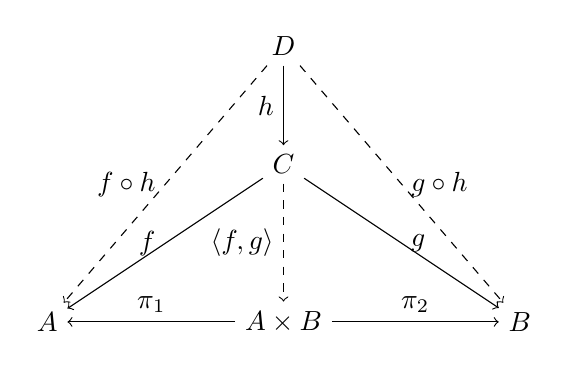
\begin{tikzpicture}
      \node (1) {$C$};
      \node[below of=1,yshift=-1cm] (2) {$A \times B$};
      \node[left of=2,xshift=-2cm] (3) {$A$};
      \node[right of=2,xshift=2cm] (4) {$B$};
      \node[above of=1,yshift=0.5cm] (5) {$D$};

      \draw[dashed,->] (1) -- node[left] {$\langle f , g \rangle$} (2);
      \draw[->] (1) -- node[left] {$f$} (3);
      \draw[->] (1) -- node[right] {$g$} (4);
      \draw[->] (2) -- node[above] {$\pi_1$} (3);
      \draw[->] (2) -- node[above] {$\pi_2$} (4);
      \draw[->] (5) -- node[left] {$h$} (1);
      \draw[dashed,->] (5) -- node[left] {$f \circ h$} (3);
      \draw[dashed,->] (5) -- node[right] {$g \circ h$} (4);
    \end{tikzpicture}
  \end{center}

  In turn, this satisfies the product construction:
  \begin{center}
    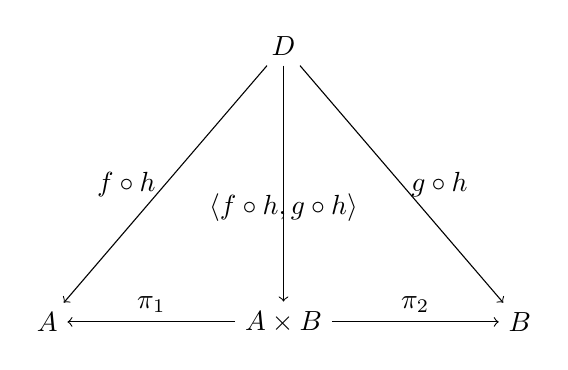
\begin{tikzpicture}
      \node (1) {};
      \node[below of=1,yshift=-1cm] (2) {$A \times B$};
      \node[left of=2,xshift=-2cm] (3) {$A$};
      \node[right of=2,xshift=2cm] (4) {$B$};
      \node[above of=1,yshift=0.5cm] (5) {$D$};

      %% \draw[dashed,->] (1) -- node[left] {$\langle f , g \rangle$} (2);
      %% \draw[->] (1) -- node[left] {$f$} (3);
      %% \draw[->] (1) -- node[right] {$g$} (4);
      \draw[->] (2) -- node[above] {$\pi_1$} (3);
      \draw[->] (2) -- node[above] {$\pi_2$} (4);
      \draw[->] (5) -- node[below] {$\langle f \circ h, g \circ h \rangle$} (2);
      \draw[->] (5) -- node[left] {$f \circ h$} (3);
      \draw[->] (5) -- node[right] {$g \circ h$} (4);
    \end{tikzpicture}
  \end{center}

  Thus the arrows $\langle f \circ h, g \circ h \rangle$ and $\langle f , g \rangle \circ h$ are equal.

\item [1.5.6.2]
\item [1.5.6.3]
\item [1.5.6.4]
\item [1.5.6.5]
\item [1.5.6.6]
\item [1.5.6.7]
\end{enumerate}
\end{document}
